\documentclass[a4paper,
			llpt,
			solution,
			accentcolor=tud2d,
			colorbacktitle
			]
			{tudexercise}

\usepackage[utf8]{inputenc}
%\usepackage[ngerman]{babel}
\usepackage{paralist}
\usepackage{amsmath}
\usepackage{pgfplots}
\pgfplotsset{compat=newest}
\usepgfplotslibrary{units}
%\usepgfplotslibrary{units}

\usepackage{multicol} \setlength{\multicolsep}{0pt}

\title{Lösungsvorschlag zur zweiten Hausübung}
\subtitle{Einführung in Net Centric Systems und \LaTeX, Sommersemester 2015}
\subsubtitle{Max Weller, Julian Haas, Stefan Pilot}

%\newcommand{\MiBs}{\frac{\mathrm{MiB}}{\mathrm{s}}}
\newcommand{\MiBs}{\mathrm{MiB}/\mathrm{s}}
\begin{document}

\maketitle
\section{}


%2.1.txt
\begin{multicols}{2}
\begin{enumerate}

\item
Normalerweise werden bei einem verbindungsorientierten Dienst die Pakete in der Reihenfolge zugestellt, in der sie gesendet wurden. Falls die Pakete in der falschen Reihenfolge beim Empfänger ankommen, werden sie entweder verworfen und später neu angefordert, oder aber gepuffert und in der richtigen Reihenfolge weitergereicht.
Es gibt allerdings Ausnahmen, z.B. das TCP-Urgent-Flag, welches den Empfänger veranlasst, ein Paket vorzuziehen.
\\\\\\
\item
Connectionless:
\begin{compactitem}
\item IP-Telefonie
\item Live-TV-Streaming
(es ist wichtig, dass Pakete mit möglichst geringer Latenz ankommen. Verloren gegangene Pakete sollten nicht wiederholt werden.)
\end{compactitem}
Connection-oriented:
\begin{compactitem}
\item Dateidownload (z.B. FTP)
(Daten müssen in der richtigen Reihenfolge und vollständig ankommen)
\item Web (HTTP)
(Webseiten und Bilder sollten in korrekter Reihenfolge übertragen werden)
\end{compactitem}
\end{enumerate}
\end{multicols}



\section{}
\subsection{}
\begin{enumerate}
\item
\begin{multicols}{2}
Während des 200ms langen Burst mit Datenrate $20\MiBs$ empfängt der token bucket 4MiB Daten: 
\begin{align*}
\text{t}_\text{burst}  \cdot \text{R}_\text{max} &= \text{Datenmenge Burst}
\\
200\mathrm{ms} \cdot 20\MiBs &= \mathrm{4MiB}
\end{align*}
Für t1 = 125ms kann der token bucket die empfangenen Daten mit $\mathrm{R}_{\mathrm{max}} = 20\MiBs$, weiterleiten:
\begin{alignat*}{5}
&\mathrm{B}     &&{}+ \mathrm{R} &&{}\cdot  \mathrm{t}_1 &&{}= \mathrm{R}_{\mathrm{max}} &&{}\cdot  \mathrm{t}_1 \\ 
& 2\mathrm{MiB} &&{}+ 4\MiBs &&{}\cdot   \mathrm{t}_1 &&{}= 20\MiBs &&{}\cdot  \mathrm{t}_1\\
&               &&{}         &&{}      \mathrm{t}_1 &&{}= 0,125\mathrm{s} &&{}
\end{alignat*}
Nach diesen 125ms verbleiben noch 1.5MiB an zu sendenden Daten:
$$4\mathrm{MiB} - \left(0.125\mathrm{s} \cdot 20\MiBs\right) = 1,5 \mathrm{MiB}$$
Diese 1.5MiB werden dann mit der Rate R = $4\MiBs
$
% = 0.004 \frac{\mathrm{MiB}}{\mathrm{ms}}$
übertragen. Das dauert 375ms:
$$
\frac{1.5 \mathrm{MiB}}{ 4 \MiBs} = 375\mathrm{ms}
$$
Die bis zur vollen Sekunde verbleibenden 500ms reichen, bis sich der token bucket wieder gefüllt hat: 
$$
4\MiBs \cdot 500\mathrm{ms} = 2\mathrm{MiB} = \mathrm{B}
$$
\vfill
\columnbreak
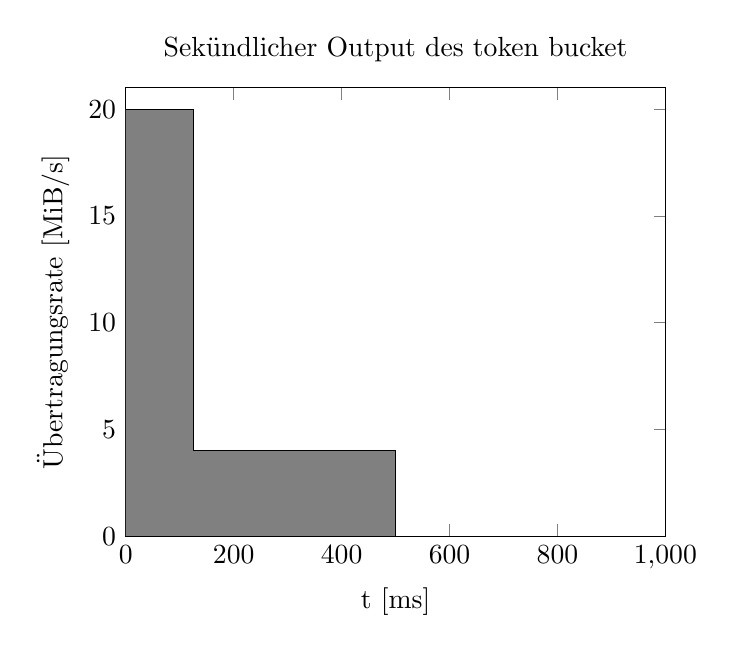
\begin{tikzpicture}
\begin{axis}[title=Sekündlicher Output des token bucket,
			 change x base,
			 x SI prefix=milli,
			 x unit=s,
			 %y SI prefix=mega,
			 xlabel=t,
			 ylabel=Übertragungsrate,
			 y unit=MiB/s,
			 ymin=0,ymax=21,
			 xmax=1,xmin=0,
			 enlargelimits=false]
			 
\addplot[const plot,fill=gray,draw=black]
coordinates {(0,20)(0.125,20)(0.125,4)(0.5,4)(0.5,0)(1,0)}
\closedcycle;
\end{axis}
\end{tikzpicture}
\end{multicols}
\newpage
\item
Während der token bucket Daten mit $20\MiBs$ versendet, füllt sich der leaky bucket mit einer Rate von
$$
20 \MiBs - 10\MiBs = 10\MiBs
$$
Nach den 125ms sind
$$
10\MiBs  \cdot 125\mathrm{ms} = 1,25 \mathrm{MiB}
$$ im leaky bucket.
In den nächsten 375ms, in denen der token bucket mit $4\MiBs$ verschickt, leert sich der leaky bucket mit einer Rate von
$$
4\MiBs - 10\MiBs = -6 \MiBs
$$
Die gespeicherten 1,25MiB Daten brauchen
$$
\frac{1.25\mathrm{MiB}}{6\MiBs} = 208.33\mathrm{ms}
$$
um den leaky bucket wieder zu verlassen.
Danach bleibt der leaky bucket bis zur nächsten vollen Sekunde leer.
\\\\
Antwort: Der leaky bucket verliert keine Daten.
\item

Wie aus den Rechnungen zu b) hervorgeht, lässt sich der Verlauf der Senderate des leaky bucket in vier Phasen aufteilen:
\begin{table}[ht]
\caption{Die vier Phasen}
\centering
\begin{tabular}{|c|c|c|c|c|}
\hline
Phase 
&
Dauer (ms)
&
Empfangsrate
&
Füllrate
&
Senderate $\left( \MiBs \right)$
\\ \hline
1 & 125\,ms    & 20\,$\MiBs$ & 10\,$\MiBs$ & 10\,$\MiBs$ \\ \hline
2 & 208,33\,ms &  4\,$\MiBs$ & -6\,$\MiBs$ & 10\,$\MiBs$ \\ \hline
3 & 166,67\,ms &  4\,$\MiBs$ &  0\,$\MiBs$ &  4\,$\MiBs$ \\ \hline
4 & 500\,ms    &  0\,$\MiBs$ &  0\,$\MiBs$ &  0\,$\MiBs$ \\ \hline
\end{tabular}
\end{table}
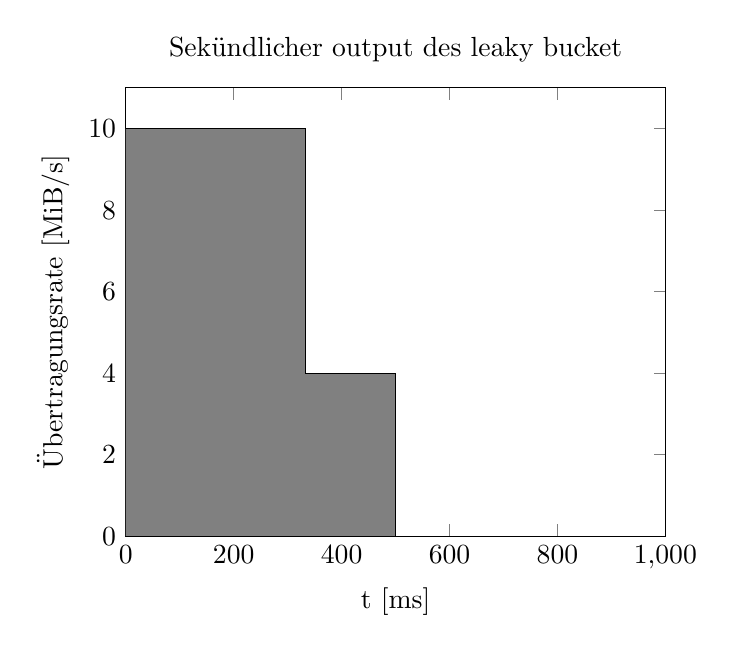
\begin{tikzpicture}
\begin{axis}[title=Sekündlicher output des leaky bucket,
			 change x base,
			 x SI prefix=milli,
			 x unit=s,
			 %y SI prefix=mega,
			 xlabel=t,
			 ylabel=Übertragungsrate,
			 y unit=MiB/s,
			 ymin=0,ymax=11,
			 xmax=1,xmin=0,
			 enlargelimits=false]
			 
\addplot[const plot,fill=gray,draw=black]
coordinates {(0,10)(0.333,10)(0.333,4)(0.5,4)(0.5,0)(1,0)}
\closedcycle;
\end{axis}
\end{tikzpicture}
\end{enumerate}
\subsection{}
\begin{enumerate}
\item
Die Füllrate des leaky bucket wird hier als $r_{fill}$ bezeichnet, die Rate, mit der der leak bucket Daten empfängt, als $r_{in}$, die in der Übung als $r$ bezeichnete Outputrate als $r_{out}$.

$$d_{bucket} = \left(r_{in} - r_{out}\right) \cdot t_{burst}$$

$r_{out}$ kann minimal $0\MiBs$ und maximal $2\MiBs$ betragen. Schon durch Einsetzen dieser Randextrema erhält man die Lösung, da der $t_{bucket}$ unter 1\,MiB liegt:

\begin{align*}
\left(15\MiBs - 0\MiBs\right) \cdot 60\mathrm{\,ms} &= 0,9\mathrm{ \,MiB}\\
\left(15\MiBs - 2\MiBs\right) \cdot 60\mathrm{\,ms} &= 0,78\mathrm{\,MiB}
\end{align*}

Antwort: r darf zwischen 0\,$\MiBs$ und 2\,$\MiBs$ betragen

\item
$$\text{DAS HIER ÜBERPRÜFEN! IST DAS WIRKLICH GEFRAGT?}$$
Bei einem Burst mit $t_{in} = 12\,\MiBs$ und einer Dauer von 120\,ms läuft der leaky bucket nach 100\,ms über.

\begin{align*}
12\, \MiBs - 2\, \MiBs \cdot t_{burst} &= 1\,\mathrm{MiB} \\
t_{burst} &= 100\,\mathrm{ms}
\end{align*}

\end{enumerate}
\section{}



\end{document}


